\section{Method}

Inspired by the rapid recent progress in instruction-tuning Large Language Models (LLMs), we choose to leverage the recently released Video Pretraining (VPT) \citep{baker2022vpt} model as a starting point for our agent. Since VPT was trained on 70k hours of Minecraft gameplay, the agent already has vast knowledge about the Minecraft environment. However, just as the massive potential of LLMs was unlocked by aligning them to follow instructions, it is likely that the VPT model has the potential for general, controllable behavior if it is finetuned to follow instructions. In this work, we present a method for finetuning VPT to follow natural, open-ended textual and visual instructions, which opens the door for a wide range of uses for VPT in Minecraft.

\begin{figure}[t]
    \centering
    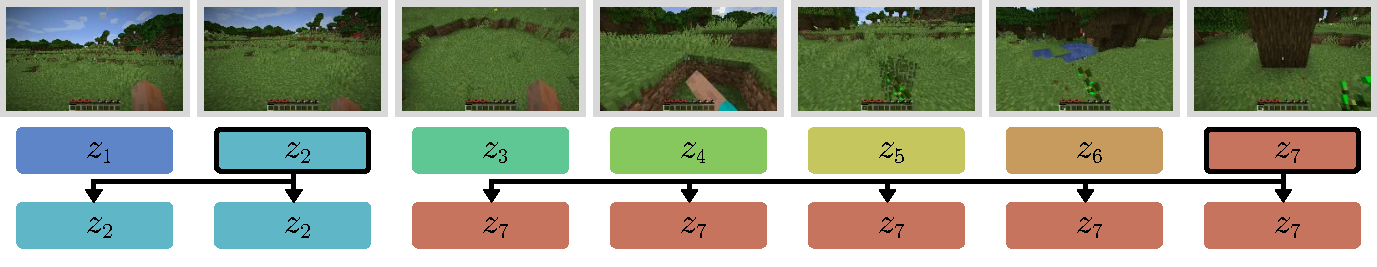
\includegraphics[width=1.0\textwidth]{figures/relabeling_diagram.pdf}
    \caption{To create goal-conditioned data for finetuning, we randomly select timesteps from episodes and use hindsight relabeling to set the intermediate goals for the trajectory segments to those visual MineCLIP embeddings. This self-supervised data teaches the agent which actions lead to which~states.}
    \label{fig:relabeling}
    \vspace{-1em}
\end{figure}

\newcommand{\zgoal}{z_{\tau_{\text{goal}}}}

Our approach is inspired by unCLIP, the method behind the recent text-to-image generation model, DALL•E 2 \citep{ramesh2022dalle2}. Our goal is to create a generative model of behavior in Minecraft conditioned on text instructions $y$. To do so, we utilize a dataset of Minecraft trajectory segments, some of which contain instruction labels $y$: $[(\tau_1, y_1), (\tau_2, y_2), \dots, (\tau_n, \emptyset)]$ where $\tau$ is a trajectory of observations and actions. We also employ a pretrained CLIP model called MineCLIP \citep{fan2022minedojo}, which generates aligned latent variables $z_{\tau_{t:t+16}}, z_y$, where $z_{\tau_{t:t+16}}$ is an embedding of any $16$ consecutive timesteps from the trajectory. MineCLIP is trained using a contrastive objective on pairs of Minecraft videos and transcripts from the web. For simplicity of notation, we refer to the MineCLIP embedding of the last 16 timesteps of a trajectory segment as $\zgoal$. Like unCLIP \citep{ramesh2022dalle2}, we utilize a hierarchical model consisting of a prior and a policy:
\begin{itemize}
    \item A \textit{prior} $p(\zgoal|y)$ that produces a latent variable $\zgoal$ conditioned on a text instruction $y$.
    \item A \textit{policy} $p(\tau|\zgoal)$ that produces a trajectory conditioned on a latent variable $\zgoal$.
\end{itemize}

These two models can then be combined to produce a generative model of behaviors conditioned on text instructions:
\begin{equation}
    p(\tau|y) = p(\tau, \zgoal|y) = p(\zgoal|y)p(\tau|\zgoal)
\end{equation}

\subsection{Policy}
To learn our policy, we finetune VPT, a foundation model of Minecraft behaviors $p_\theta(\tau)$ trained on 70k hours of Minecraft gameplay videos. Specifically, VPT consists of a ResNet \citep{resnet} that processes frames of dimension $128 \times 128 \times 3$, and a Transformer-XL \citep{txl} which processes the frame representations and autoregressively predicts the next action using the joint hierarchical action space described in \citet{baker2022vpt}. In order to modify the architecture to condition on goal information, we add an affine transformation of $\zgoal$ to the output of the ResNet before passing it to the transformer:
\begin{align*}
    \text{Process Frames:} \quad & \text{ResNet}_{\theta}(o_t) \rightarrow x_t \\
    \text{[+ Conditioning on MineCLIP Embedding Goal]:} \quad & x_t \rightarrow x_t + W_{\theta} \zgoal + b_{\theta} \\
    \text{Predict Actions:} \quad & \text{TransformerXL}_{\theta}(x_t, \ldots, x_{t+T}) \rightarrow a_{t+T}
\end{align*}

In order to finetune VPT to condition on goals, we finetune the model using a method inspired by supervised RL approaches like Decision Transformer \citep{chen2021decision}, GLAMOR \citep{paster2020planning}, and GCSL \citep{ghosh2021gcsl}. We use a modification of hindsight relabeling which we call \textbf{packed hindsight relabeling} (see \autoref{fig:relabeling}) to generate a new dataset of trajectories with goals pulled from future states that periodically switch. In contrast with hindsight relabeling, packed hindsight relabeling packs multiple relabeled sequences into a single sequence. Specifically, our method to generate this dataset consists of two steps:
\begin{enumerate}
    \item Given a trajectory $\tau$ with $T$ timesteps, randomly generate indices to select goals from: $i_1, i_2, \ldots, i_n$. These indices are chosen by starting at the first timestep and repeatedly sampling a new timestep by adding a random value to the previous timestep. This ensures that the data reflects that some goals may take longer to achieve than others.
    \item For each chosen goal at timestep $i_j$, set the goals for timesteps $i_{j-1} + 1, \ldots, i_j$ to be the goal at timestep $i_j$, denoted $z_{\tau_{i_j}}$.
\end{enumerate}

\newcommand{\drelabeled}{\mathcal{D_{\text{relabeled}}}}

Our final dataset $\drelabeled$ consists of observation sequences $(o_1, \ldots, o_T)$, action sequences $(a_1, \ldots, a_T)$, and packed hindsight relabeled goals $(z_1, \ldots, z_T)$. We then finetune VPT on this dataset using a supervised loss to predict each action autoregressively using a causal attention mask:
\begin{equation}
    \mathcal{L}_{\text{policy}}(\theta) = \E_{\drelabeled}\left[-\log p_{\theta}(a_t|o_{1\ldots t}, z_{1\ldots t})\right]
\end{equation}

\subsection{Prior}

\newcommand{\dlabeled}{\mathcal{D_{\text{labels}}}}

In order to condition not only on embeddings of visual goals but on latent goals, we need the prior, a model that produces a latent variable $\zgoal$ conditioned on a text instruction $y$. Our model is a simple conditional variational autoencoder (CVAE) \citep{cvae,vae} with a Gaussian prior and a Gaussian posterior. Rather than learn to condition directly on text, we choose to condition on frozen text representations from MineCLIP $z_y$. Thus, the prior learns a function to translate from a text embedding $z_y$ to a visual embedding $\zgoal$ (see \Cref{appendix:gen_to_novel_text} for further discussion). Both the encoder and decoder of our CVAE are parameterized as two-layer MLPs with 512 hidden units and layer normalization \citep{ba2016layer}. We train the model on our dataset, for which we have text labels $\dlabeled$ using the following loss:
\begin{equation}
    \mathcal{L}_{\text{prior}}(\phi) = \E_{(\zgoal, z_y) \sim \dlabeled}\left[\KL{q_{\phi}(\zgoal|z_y)}{p(\zgoal)} - \E_{c \sim q_{\phi}(\zgoal|z_y)}\left[\log p_{\phi}(\zgoal|c, z_y)\right]\right]
\end{equation}

\subsection{Datasets}
\label{sec:prior_dataset}
To train our policy, we gather a gameplay dataset with 54M frames ($\approx 1$ month at 20FPS) of Minecraft gameplay along with associated actions from two sources: contractor gameplay and VPT-generated gameplay. To train our prior, we use a small dataset of text-video pairs gathered by humans and augmented using the OpenAI API \texttt{gpt-3.5-turbo} model~\citep{chatgpt} and MineCLIP. See \autoref{appendix:datasets} for more detailed dataset information.

\paragraph{OpenAI Contractor Dataset} We use 39M frames sourced from the contractor dataset which VPT \citep{baker2022vpt} used to train its inverse dynamics model and finetune its policy. The dataset was gathered by hiring human contractors to play Minecraft and complete tasks such as house building or obtaining a diamond pickaxe. During gameplay, keypresses and mouse movements are recorded. We use the same preprocessing as VPT, including filtering out null actions.

\paragraph{VPT-Generated Dataset} We generate an additional dataset of 15M frames by generating random trajectories using the various pretrained VPT agents. The diversity of this dataset is improved by randomly switching between models during trajectories \citep{paster2022return}, randomly resetting the agent's memory, and randomly turning the agent to face a new direction.

\paragraph{Text-Video Pair Dataset} To train our prior model, which learns a mapping between text embeddings and visual embeddings, we also manually gather a small dataset of 2,000 text instructions paired with 16-frame video segments (less than a second) from our gameplay dataset. This dataset corresponds to less than 30 minutes of gameplay and takes just a few hours to collect. We augment this dataset by using the alignment between text and video embeddings from MineCLIP. For each text instruction, we find the top $k$ most similar gameplay segments in our dataset and use the corresponding 16-frame segment as additional training data. For augmentation, we also add 8,000 text-instructions generated by the OpenAI API \texttt{gpt-3.5-turbo} model~\citep{chatgpt}, in addition to our 2,000 hand-labeled instructions.

\subsection{Inference}
\label{sec:inference}

At inference time, we use the prior to sample a latent goal $\zgoal$ from the text instruction $y$. We then use the policy to autoregressively sample actions $a_t$ conditioned on the observation history $o_{1\ldots t}$ and the latent goal $\zgoal$. Similar to the observation in Appendix I of \citet{baker2022vpt}, even with conditioning, the policy often fails to follow its instruction and simply acts according to its prior behavior. To mitigate this, we borrow another trick used in image generation models: classifier-free guidance. Specifically, during inference we simultaneously compute logits for the policy conditioned on the goal $f(o_t, \ldots, o_{t+1}, \zgoal)$ and for the unconditional policy $f(o_t, \ldots, o_{t+1})$. We then compute a combination of the two logits using a $\lambda$ parameter to trade-off between the two:

\bigskip
\begin{equation}
    \operatorname{logits} = (1 + \lambda) \underbrace{f_{\theta}(o_t, \ldots, o_{t+1}, \zgoal)}_{\text{conditional logits}} - \lambda \underbrace{f_{\theta}(o_t, \ldots, o_{t+1})}_{\text{unconditional logits}}
\end{equation}
By setting a higher value of $\lambda$, we can encourage the policy to follow actions that are more likely when conditioned on the goal and, as demonstrated in \Cref{par:cfg}, this significantly improves performance. Also, in order to train the policy to generate these unconditional logits, we occasionally dropout the goal embedding $\zgoal$ from the policy's input (with probability 0.1). This lets us generate both the conditional and unconditional logits using the same model with batch processing at inference time.

\subsection{Evaluation}

Evaluating the performance of our agent is a challenging task due to the wide variety of instructions that are possible and the difficulty of evaluating whether the agent has successfully achieved its task. We use a combination of programmatic evaluation metrics and automatic MineCLIP evaluation metrics to get a sense of the agent's capability level. We collectively refer to all of our evaluation tasks including the 11 evaluation tasks from \autoref{fig:final_perf} and the two prompt chaining tasks from \Cref{sec:exp_chaining} as our \textit{early-game evaluation suite}.

\paragraph{Programmatic Evaluation}

We compute programmatic evaluation metrics by monitoring the MineRL \citep{guss2019minerl} environment state throughout each evaluation episode. As done in VPT \citep{baker2022vpt}, we compute multiple programmatic metrics including travel distance and early-game item collection. The travel distance is the maximum displacement of the agent along on the horizontal (X-Z) plane, measured from the initial spawn point. For early-game inventory counts, we store the maximum number of log, seed, and dirt items seen in the agent's inventory during the episode. 

\paragraph{MineCLIP Evaluation}

We explore the use of text-visual alignment in MineCLIP latent space between trajectories and text or visual goals to evaluate our agent over a wider variety of tasks where programmatic evaluation isn't practical. To determine the degree to which a task has been completed at all during an evaluation episode, we record the minimum cosine distance between the (text or visual) goal embedding and the visual MineCLIP embedding at any timestep during an episode.
